%% USPSC-Cap2-Desenvolvimento.tex 

% ---
% Este capítulo, utilizado por diferentes exemplos do abnTeX2, ilustra o uso de
% comandos do abnTeX2 e de LaTeX.
% ---

\chapter{Desenvolvimento}\label{cap_exemplos}

\section{Revisão sistemática}
O estudo de Revisão Sistemática da Literatura seguiu as recomendações Preferred Reporting Items for Systematic Reviews and Meta-Analisys – PRISMA.
Foram buscados os termos: “patent mining”, “patent”, “random forest”, “machine learning” - nas seguintes bases de dados: Periodicos CAPES, Microsoft research, Semantic Scholar e Google Scholar. O intervalo de publicação dos artigos selecionados estão entre 2012 a 2020 e restrito a somente artigos escritos em inglês.

\subsection{Descrição do objeto de estudo}
Foi realizado a extração de dados de documentos de patentes no site Free Patents Online - FPO (https://www.freepatentsonline.com/). Este site contem os dados dos documentos de patentes de forma pública.

\subsection{Delineamento da pequisa}
Foi buscado o termo “agronomy” e filtrado para somente documentos de patentes registrados nos Estados Unidos. Foi totalizado 12906 patentes, dos quais selecionamos uma amostragem das 200 primeiras patentes. Construímos uma aplicação de webscraping na linguagem Python para realizar a extração dos dados de documentos de patentes.  Os dados extraídos foram armazenados em um banco de dados.

\section{Materiais e métodos}

\subsubsection{Extração dos dados}
A aplicação de webscraping dos dados de documentos de patentes foi escrita na linguagem de programação Python, com uso das bibliotecas \textit{requests} e \textit{BeautifulSoup}. Essa aplicação é modular o suficiente para que seja definido quantos documentos de patentes terão suas informações extraídas, como também quais informações serão extraídas, como demonstrado na figura \ref{webscraping_flow_image}. Os dados são organizados na forma de tabela e armazenado em um pequeno banco de dados feito em \textit{SQLite}.

\begin{figure}[ht!]
	\centering
	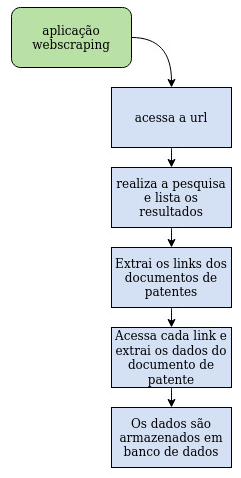
\includegraphics[scale=0.5]{imagens/tcc_webscraping.jpg}
	\caption{Fluxo de captura dos dados de documentos de patente 
			 \label{webscraping_flow_image}}
\end{figure}


\subsubsection{Construção do dicionario}
A construção do dicionario que será utilizado no projeto é composto pelas seguintes etapas, figura \ref{dicionario_flow_image}, geração de um corpora de documentos de patentes, pre processamento do corpora, obtenção da matriz de documento-termo (Document-Term Matrix – DTM) e aplicação do modelo Latent Dirichlet allocation (LDA). A partir dos tópicos apresentados pelo resultado do LDA, são adicionados ao tópicos, palavras relacionadas, tais como sinônimos, hiperônimos e hipônimos através do banco de dados wordnet.

\begin{figure}[ht!]
	\centering
	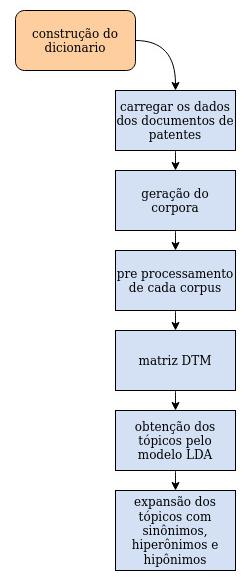
\includegraphics[scale=0.5]{imagens/tcc_dicionario.jpg}
	\caption{Fluxo de criação do dicionario
			 \label{dicionario_flow_image}}
\end{figure}

\subsection{Validação do dicionario}
A avaliação do dicionario obtido, consiste em observar se o valor k utilizado para geração de tópicos conseguiu separar adequadamente os assuntos contidos no corpora.

\section{Resultados parciais}

\subsection{Extração de dados}

Extraímos uma amostra no total de 200 documentos de patentes através do uso da técnica de webscraping. Destes documentos, os dados de \textbf{Titulo} e \textbf{Resumo} foram pré processados, removendo as quebras de linhas, espaços no inicio e fim da frase, uso de somente um espaço como separador e transformação em minusculo. Estes dados foram concatenados e usados para a montagem do corpora de documentos de patentes, que poderá ser utilizado para outros projetos.

\begin{figure}[ht!]
	\centering
	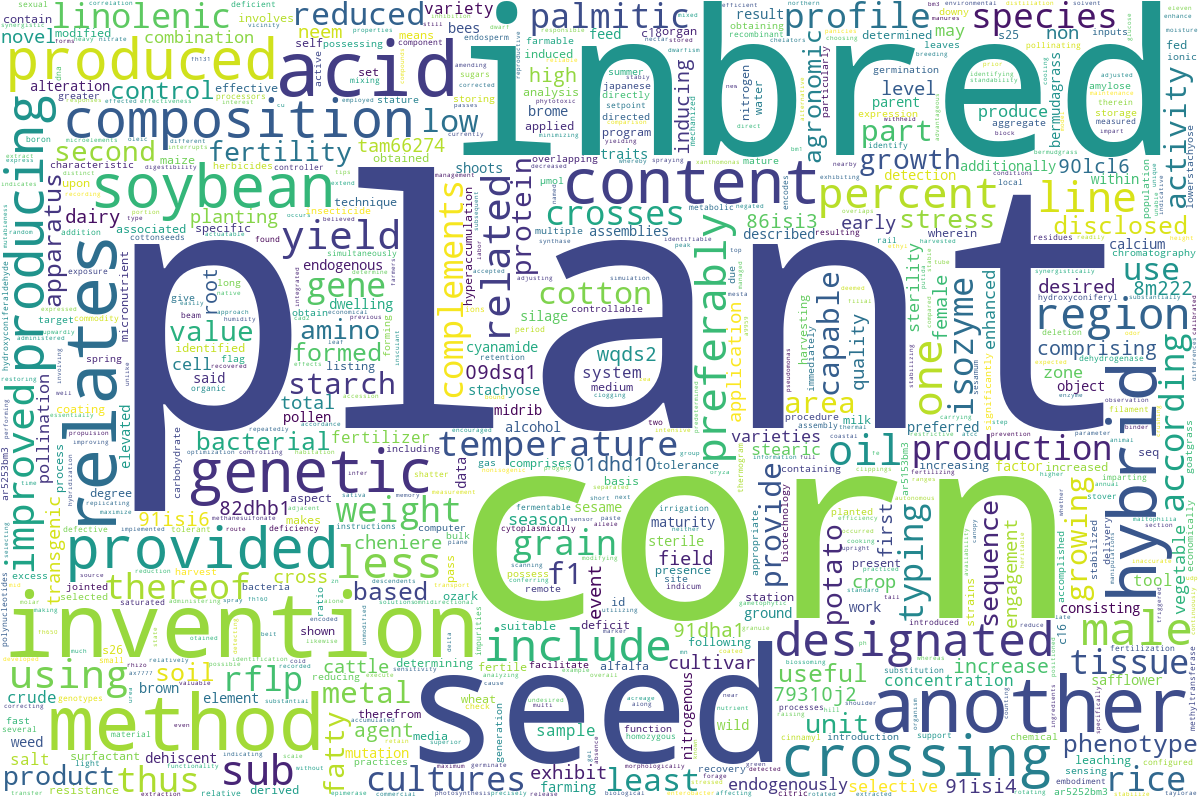
\includegraphics[scale=0.3]{imagens/wordcloud_preprocess.png}
	\caption{Construção nuvem de palavras dos termos mais representativas para este corpora.
			 \label{wordcloud_pre_image}}
\end{figure}

\subsection{Construção do dicionario}

A construção do dicionario engloba o levantamento de tópicos, expansão dos termos, avaliação dos tópicos e expansão dos termos.

\subsubsection{Levantamento de tópicos}

O corpora de documentos de patentes foi carregado, removido as \textbf{stopwords}, removido também caracteres numéricos e especiais, depois separados em palavras (tokens) e convertidos em sua raiz (lemmas). Resultando em 200 conjuntos de palavras normalizadas representando cada documento de patente e que esta pronto para ser utilizado em modelos de Processamento de Linguagem Natural e em modelos de Aprendizado de Maquina.
Aplicamos o modelo LDA, com os seguintes parâmetros - random\_state igual a 100, update\_every igual a 1, chuncksize igual a 100, passes igual a 10 e alpha automático. Para definir a quantidade de tópicos k, usamos um laço de 40 interações e anotamos o valor da métrica Coherence.

\begin{figure}[ht!]
	\centering
	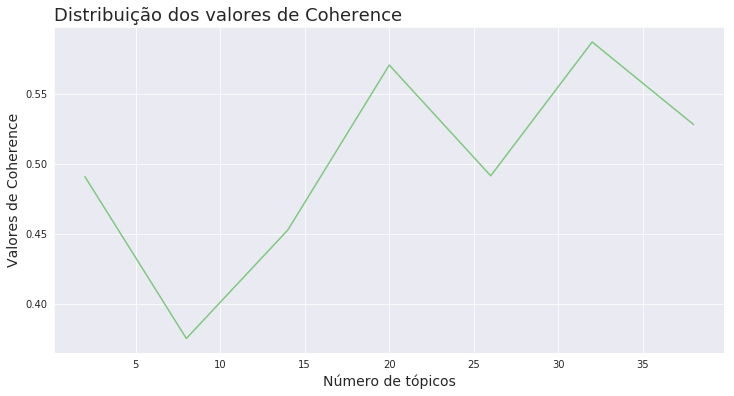
\includegraphics[scale=0.6]{imagens/distr_dos_valores_de_coherence.png}
	\caption{A distribuição dos valores de Coherence ao longo da variação do parametro k, permite que observemos qual a quantidade de tópicos devemos ter.
			 \label{dist_coherence_image}}
\end{figure}

O gráfico aponta que um k igual a 20 resulta no segundo mais alto valor de Coherence. Utilizaremos este valor para k, pois é um número menor de conjuntos de palavras que precisará serem interpretadas para se definir qual o título do tópico se referem.

\subsubsection{Validação dos tópicos}

Examinamos o tópicos obtidos através da ferramenta pyLDAvis. Os termos que compõe os tópicos gerados  representam bem o corpora usado. Temos pouca sobreposição, com exceção do tópico 18, e os termos de cada tópico possuem uma alta relevância com o tema agronomia.  

\begin{figure}[ht!]
	\centering
	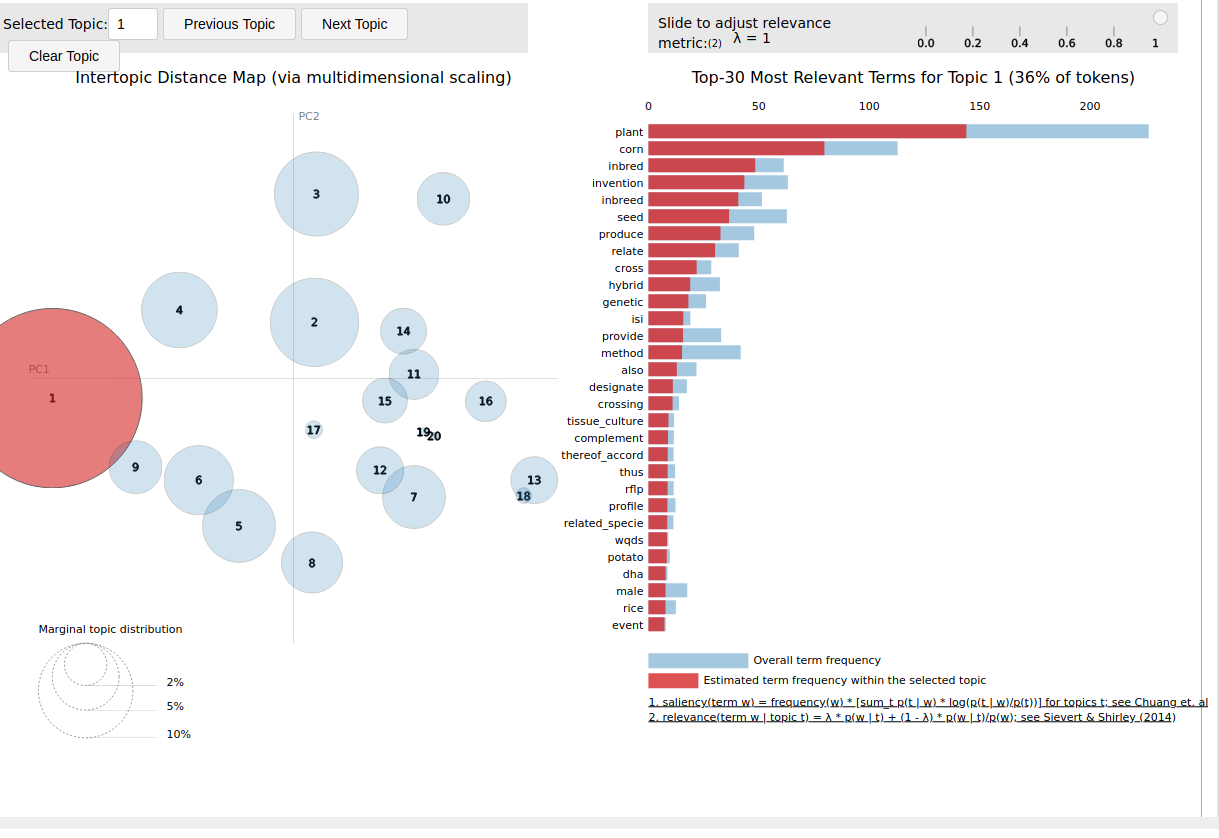
\includegraphics[scale=0.4]{imagens/construcao_dicionario1.png}
	\caption{O grafico de bolhas, cada bolha representa um tópico, o tamanho da bolha representa a prevalencia do tópico e a sobreposição de bolhas aponta a similaridade entre os tópicos. O gráfico da direita, as barras representam a relevância do termo para o tópico observado.
			 \label{pyLDAvis_image}}
\end{figure}

\subsubsection{Expansão do dicionário}

Os tópicos geraram no total de 119 palavras únicas que foram submetidas ao wordnet e adicionado os sinônimos, hiperônimos e hipônimos destes termos, totalizando 673 termos que representam cada tópico.

\section{Discussão parcial}

Conseguimos realizar a extração bem sucedida de uma amostra de documentos de patentes, do qual pré processamos e criamos um corpora que poderá ser usado não somente para este trabalho como para outros trabalhos com documentos de patentes. Fizemos um primeiro levantamento dos tópicos usando o modelo LDA e obtivemos 20 tópicos que serão avaliados e rotulados corretamente. 
Utilizando termos simples para rotular os tópicos neste primeiro momento, expandimos com termos que são sinônimos, hiperônimos e hipônimos dos termos associados aos tópicos. 

Para os próximos passos, desenvolveremos um modelo para classificar os documentos de patentes a partir do dicionario criado. 

